%Report Structure =============================================================
%Introduction
%		Chapter 1 Introduction
%Fundamentals
%		Chapter 2 State of the Art
%Contributions
%		Chapter 3 
%   Chapter 4 
%Topic2
%   Chapter 5 
%Experiments
%		Chapter 6 The Experimental Robotic Platform
%		Chapter 7 Experiments
%Conclusions
%		Chapter 8 Conclusions and Future Outlook
% References
%==============================================================================

\documentclass[12pt,BCOR=1cm,bibliography=totoc]{thesis}
\pdfminorversion=5 
\pdfcompresslevel=9 
\pdfobjcompresslevel=3
%\usepackage{showframe}

%\KOMAoptions{headings=small}
%\addtokomafont{disposition}{\rmfamily\mdseries}
%\renewcommand*{\contentsname}{Table of Contents}
%\setkomafont{chapterprefix}{\rmfamily\Large\bfseries}


% customize chapter format:
\KOMAoption{headings}{twolinechapter}
\renewcommand*\chapterformat{\color{blue}{Chapter \thechapter}\vspace{-0.6cm}}%\autodot

% customize dictum format:
\setkomafont{dictumtext}{\itshape\small}
\setkomafont{dictumauthor}{\tiny}
\renewcommand*\dictumwidth{0.5\linewidth}
\renewcommand*\dictumauthorformat[1]{--- #1}
\renewcommand*\dictumrule{}


\usepackage{float}
\usepackage{pdfpages}

%*****************************************************************************
\graphicspath{ {figures/} }

%** new commands ******************************************************
%!TEX root = myThesis.tex
%!TEX encoding = UTF-8 Unicode

%***************************************************************************************************
% create smaller pdf
% http://tex.stackexchange.com/questions/14429/pdftex-reduce-pdf-size-reduce-image-quality

%  gs -sDEVICE=pdfwrite -dCompatibilityLevel=1.4 -dPDFSETTINGS=/prepress -dNOPAUSE -dQUIET -dBATCH -sOutputFile=small.pdf Doktorarbeit.pdf

%  gs -sDEVICE=pdfwrite -dCompatibilityLevel=1.4 -dPDFSETTINGS=/ebook -dNOPAUSE -dQUIET -dBATCH -sOutputFile=small.pdf Doktorarbeit.pdf

% -dPDFSETTINGS=/screen   (screen-view-only quality, 72 dpi images)
% -dPDFSETTINGS=/ebook    (low quality, 150 dpi images)
% -dPDFSETTINGS=/printer  (high quality, 300 dpi images)
% -dPDFSETTINGS=/prepress (high quality, color preserving, 300 dpi imgs)
% -dPDFSETTINGS=/default  (almost identical to /screen)
%***************************************************************************************************


% settings -------------------------------------------------------------------
%try this to fix the margin problem
%http://tex.stackexchange.com/questions/10128/two-sided-document-reverse-page-margins-for-hardcopy
%***************************************************************************************************

\usepackage{mathtools} %for the dcases environment
%*****************************************************************************
\setlength{\marginparwidth}{0pt}

\newenvironment{myCompactItemize}
{ \begin{itemize}
    \setlength{\itemsep}{0pt}
    \setlength{\parskip}{0pt}
    \setlength{\parsep}{0pt}     }
{ \end{itemize}                  } 

% 'text' shortcuts -----------------------------------------------------------
\newcommand{\etal}{\textit{et al.\ }}
\newcommand{\kmeans}{$k$--{\ttfamily means} }
\newcommand{\kmeanspp}{$k$--{\ttfamily means++} }
\newcommand{\art}{\textit{i}{\scshape ArteC} }

% math stuff -----------------------------------------------------------------
\DeclareMathOperator{\sgn}{sgn}
\DeclareMathOperator*{\argmin}{arg\,min}
\newcommand{\s}[2]{\left\langle #1,#2\right\rangle} % scalar product
\newcommand{\n}[1]{\left\|#1\right\|}  							% norm
\newcommand{\abs}[1]{\left |#1\right |} 						%abs, magnitude


%commented out because it causes  the error:
%too many math alphabets used in version normal
%\usepackage{bm}
%\renewcommand{\vec}[1]{\ensuremath{\bm{#1}}}
%\newcommand{\matx}[1]{\ensuremath{\bm{#1}}}     		%matrix notation (ISO complying version)

\renewcommand{\vec}[1]{\ensuremath{\mathbf{#1}}} 	%vector notation
\newcommand{\matx}[1]{\ensuremath{\mathbf{#1}}} 		% matrix notation


%$\begin{bmatrix*}[r]
  %-1 & 3 \\
  %2 & -4
 %\end{bmatrix*}
%$

% environment redefenitions --------------------------------------------------
\newtheorem{defn}{Method}%{\bfseries}{\itshape}
\theoremstyle{definition} %plain | definition | remark
\newtheorem{definition}{Definition}

%shorthand for the nomenclature that prints the symbol/abbreviation and generates a list entry at the same time.
\newcommand*{\nom}[2]{#1\nomenclature{#1}{#2}}
%example: \nom{EST}{Eastern Standard Time}
%\nom{}{}

%\def\mydate{\leavevmode\hbox{\the\year-\twodigits\month-\twodigits\day}}
\def\mydate{\leavevmode\hbox{\the\year\twodigits\month\twodigits\day}}
\def\twodigits#1{\ifnum#1<10 0\fi\the#1}

%** listings settings ******************************************************

\lstset{basicstyle=\footnotesize\ttfamily,breaklines=true}
\lstset{framextopmargin=50pt,frame=bottomline}
\lstset{showstringspaces=false}%do not use "squat-u" symbole for space

\lstdefinelanguage{XML}{ 
    columns=fullflexible, 
    basicstyle=\footnotesize\ttfamily, 
    commentstyle=\ttfamily\color{green!50!black}, 
    morestring=[s]{"}{"}, 
        alsoletter={ },
    morecomment=[s]{?}{?}, 
    morecomment=[s]{!--}{--}, 
    morecomment=[s]{!DOCTYPE}{]}, 
    moredelim=[s][\color{black}]{>}{<}, 
    moredelim=[s][\bfseries\color{black}]{\ }{=}, 
    stringstyle=\color{blue}, 
    identifierstyle=\bfseries\color{violet} 
} 

\lstdefinelanguage{terCmd}{
        basicstyle=\footnotesize\ttfamily, 
    sensitive=false,
    alsoletter={.},
    alsoletter={\$},
    morestring=[s]{"}{"}, 
    stringstyle=\color{blue}, 
    morestring=[s]{'}{'}, 
    %stringstyle=\color{violet}, 
    moredelim=[s][\color{red}]{<}{>},
    moredelim=[s][\color{blue}]{[}{]},
    %  moredelim=[is][\color{orange}]{:}{:},
    keywords=[10]{roslaunch,model,rospack,find,source,cd,sudo,usermod,chmod},
    keywordstyle=[10]{\color{magenta}},
}

\lstset{language=C++,
    basicstyle=\footnotesize\ttfamily,
    keywordstyle=\color{blue}\ttfamily,
    stringstyle=\color{red}\ttfamily,
    commentstyle=\color{teal}\ttfamily,
    morecomment=[l][\color{magenta}]{\#}
}

\begin{document}
\pagestyle{empty}
%\titlehead{\centering\includegraphics[width=0.15\textwidth]{myFrontMatter/figures/zuLogo}
%    
\includegraphics[width=0.2\textwidth]{myFrontMatter/figures/engLogo}}
\begin{titlepage}
\centering
\includegraphics[width=0.15\textwidth]{myFrontMatter/figures/zuLogo} \qquad 
\includegraphics[width=0.2\textwidth]{myFrontMatter/figures/engLogo}\\
{\usekomafont{titlehead}   Zagazig University, Faculty of Engineering,\\Computer and Systems Engineering Dept.}

  \vskip 10ex
{\LARGE\usekomafont{title} {\LARGE  ZagHexa: Design, Construction and Control of a Hexapod Walking Robot} }
\vskip 8ex
\emph{Graduation project for the degree Bachelor of Science (B.Sc.)\\
Submitted to Computer and Systems Engineering Dept., Faculty of Engineering, Zagazig University, Egypt}

\vskip 8ex
{\usekomafont{subtitle} By}
\vskip 1ex
{\usekomafont{author} 
    Mahmoud Mohammed Elsayed\\
    Khaled Mohammed  Risha\\
    Mohammed Alaa Mohammed\\
    Hend Khairy Abdelhamed\\
    Nehad Abdelsalam Mohammed\\
    Amira Elsayed Soliman
}

\vskip 6ex
{\usekomafont{subtitle} Supervisor}
\vskip 1ex

{\usekomafont{author}
    \emph{\normalsize  Asst. Prof. Dr.Ing.}\\
    \textbf{Mohammed Nour A. Ahmed} \\
     {\itshape\small Computer and Systems Engineering Dept.\\
    Faculty of Engineering, Zagazig University, Zagazig, Egypt}
}

\vfill
July, 2017
\end{titlepage}
%%% Rückseite der Titelseite %%%%%%%%%%%%%%%%%%%%%%%%%%%%%%%%%%%%%%%%%%%
%\uppertitleback{Graduation Project Report to be submitted to\\
%Zagazig University, faculty of Engineering\\
%in partial fulfillment of the requirements for the degree \\
%Bachelor of Science in Engineering (B.Sc.)\\
%\textcopyright 2017\\
%
%\vspace{2cm}
%   {\footnotesize
%      Copyright \textcopyright 2017 Dr.Ing. Mohammed Nour Abdelgwad Ahmed as part of the course work and learning material. All Rights Reserved. 
%      Where otherwise noted, this work is licensed under 
%      \href{https://creativecommons.org/licenses/by-nc-sa/4.0/}{ a Creative Commons Attribution-NonCommercial-ShareAlike 4.0 International License}.}
% 
\includegraphics[width=0.2\textwidth]{byncsa}
%
%}
%
%
%
%\lowertitleback{\textbf{Date of Presentation}\\
%  18. July 2017\\~\\
%  
%  \textbf{Supervisors}\\
%Dr.Ing. \textbf{Mohammed Nour Abdel Gwad Ahmed}\\
%\footnotesize{\itshape 
% Computer and Systems Engineering Department,\\
%  Faculty of Engineering, Zagazig University, Egypt}\\~\\
%
%
%%\textbf{Defense Commete}\\
%%Prof. Dr. Xyz Wuv\\
%%Prof. Dr. Abc Def
%}
%

%% Rückseite der Titelseite %%%%%%%%%%%%%%%%%%%%%%%%%%%%%%%%%%%%%%%%%%%
\newpage
{Graduation Project Report submitted to\\
    \textbf{Zagazig University, faculty of Engineering, Computer and Systems Engineering Department}, Zagazig, Egypt\\
    in partial fulfillment of the requirements for the degree \\
    Bachelor of Science in Engineering (\textbf{B.Sc.})\\
    \textcopyright 2017\\~\\
    
      \vspace{1cm}
    {\footnotesize
        Copyright \textcopyright 2017 Asst. Prof. Dr.Ing. Mohammed Nour Abdelgwad Ahmed as part of his course work and learning material. All Rights Reserved. 
        Where otherwise noted, this work is licensed under 
        \href{https://creativecommons.org/licenses/by-nc-sa/4.0/}{ a Creative Commons Attribution-NonCommercial-ShareAlike 4.0 International License}.}\\
    
\includegraphics[width=0.15\textwidth]{myFrontMatter/figures/byncsa}}\\

  \vspace{1cm}
{\textbf{Date of Presentation}\\
  18. July 2017\\~\\
    
    
    
    {\textbf{Project Team Members}\\
        \noindent\begin{tabular}{ll}
             Mahmoud Mohammed Elsayed&        Khaled Mohammed  Risha\\
            Mohammed Alaa Mohammed&            Hend Khairy Abdelhamed\\
            Nehad Abdelsalam Mohammed&        Amira Elsayed Soliman
        \end{tabular}\\~\\
        
        \textbf{Project Leader}\\
        Asst. Prof. Dr.Ing. \textbf{Mohammed Nour A. Ahmed}\\
        {\itshape \footnotesize
            Computer and Systems Engineering Department,\\
            Faculty of Engineering, Zagazig University, Egypt}\\~\\
       
        
        
      
        \vfill
        {\tiny Revision git.198.50.\mydate   % get git version number to be used as the version no. of the doc.
            \immediate\write18{./myGitVer.sh.command \jobname.txt}
            Version: \input{\jobname.txt}}
    }

\dedication{to\\
%$\mathfrak{Yasmin}$, 
%$\mathfrak{Nour}$, 
%$\mathfrak{Adham}$, and 
%$\mathfrak{Lena}$.\\
\textbf{All}, \textbf{Whom}, \textbf{we}, and \textbf{love}.\\
The best in my life and after ...}
\maketitle 						% Titelei wird erzeugt

\frontmatter %-------------------------------------------------------------
\pagestyle{fancy}

%\include{myFrontMatter/abstractEn}%\cleardoublepage{}
%\include{myFrontMatter/abstractAr}%\cleardoublepage{}
\markboth{Abstract}{}
\addcontentsline{toc}{chapter}{Abstract}
\chapter*{Abstract}
This report is a documentation of the final year graduation project in electrical engineering at zagazig university. The purpose of this project is to Design, Construction and Control of a six-legged walking robot that is capable of basic mobility tasks such as walking forward, backward, rotating in place and raising or lowering the body height.

The legs are of a modular design that have three degrees of freedom each. This robot will serve as a platform onto which additional sensory components could be added, or which could be programmed to perform increasingly complex tasks.

The components that make up our final design are discussed. Also, we describe the basic robot gaits of locomotion for efficient navigation. This locomotion is tuned to make the robot faster and at same time energy efficient to navigate and negotiate difficult terrain.

The robot is an integrated multi-legged walking robot based on de-facto standard Robotic Operating System (ROS) that employs novel and different walking patterns.

Our robot is teleoperated using hand-held devices such as a smart phone or tablet or a wireless joystick. Furthermore, it has its own navigation system and a camera for instant video recording and streaming.

The power to the entire system is supplied through two 5 volts NiMH batteries. There is an additional power bank to power up the Raspberry Pi and other electronic components. 
We have an interactive website for robot inspection and online control in addition to leaning materials such as robot building and implementation walkthroughs and as well as step-by-setup tutorials.\\


\textbf{Keywords} -- biologically inspired, legged robot, gait generation, design procedure, simulation


\markboth{Acknowledgements}{}

\chapter*{Acknowledgements}
\addcontentsline{toc}{chapter}{Acknowledgements}

This graduation project consumed huge amount of work, research and dedication. Still, accomplishment would not have been possible if we did not have a support of many individuals. Therefore we would like to extend our sincere gratitude to all of them.

%advisor
First of all, we would like to sincerely thank our advisors Dr.Ing. Mohammed Nour and Dr Ahmed Hamdy. They gave us the opportunity to work on great ideas with great people . When needing someone for the
discussion of any problem, ..... was always there and also solved a lot of .......... problems for/with us.



we are also grateful to our friends and colleagues, XYZ, ABC, and UVW. For getting into the basics of this project, we had a lot of support by XYZ who raised our first interest during the initial part of this work. ABC helped us a lot with the .........  and experiments. UVW helped so much in ......... We are indebted to ........... for making ............. easier to understand and to introduce ........ to us. 

%Experiments: 
we express our warm thanks to ......, ............., and ............. for making the ............. robot available to us and the time they spend assisting us to carry out the field experiments. Without their superior knowledge and experience, the experiments would not have that like in quality of outcomes, and thus their support has been essential. In addition, we wish to express our sincere gratitude to ............. for helping when we had questions as well as frustrations.


We would like to thank all the numerous people in the internet who ask questions and provide answers for programming problems (specifically in ROS) and for the very useful code and tools they share with others.

%family and friends
we would like to most importantly acknowledge the effort of our families, who encouraged us to pursue higher education and support us through the difficulties associated with such a goal even when we was not sure we would make it through. 

Last but not least, we would like to thank our friends for always encouraging us onwards. We can
never thank them enough for their love and faith.

%Egypt
This work was supported by a financial aid  from Zagazig University. We would like to thank the funders. They had no role in study design, data collection and analysis, decision to publish, or preparation of this work.
%\cleardoublepage{}

\tableofcontents
\listoffigures
%\begin{minipage}[b]{1\linewidth}
   %\listoftables
%\end{minipage}
%\begin{minipage}[b]{1\linewidth}
     %\listofalgorithms
%\end{minipage}
\listoftables
\listofalgorithms


\chapter*{Key abbreviations}

\begin{tabular}{l    l }
    DOF & Degree of freedom  \\  
    PWM &  Pulse Width Modulation  \\   
    $I^2C$  & Inter-Integrated Circuit   \\  
    Hexapod &  six-leg walking robot \\  
    DMP & Digital Motion Processor \\  
    LiPo &   Lithium Polymer\\ 
    RPM   & Round Per Minute  \\
    RPi &   Raspberry Pi\\  
    GPIO &  General-purpose input/output \\  
    ADC   & Analog-Digital Converter   \\  
    LPF & Low Path Filter \\
    HPF &  High Path Filter \\
    FPS & Frame Per Seconds\\
    GND & Ground
\end{tabular} 


\mainmatter %-----------------------------------------------------
\pagestyle{fancy}
%------------------------------------------------------------------


\setchapterpreamble[o]{%
    \dictum[Niccolo Machiavelli, \textit{(Italian writer and statesman, Florentine patriot, author of 'The Prince', 1469-1527)}]{%
        ``There is nothing more difficult to take in hand, more perilous to conduct or more uncertain in its success than to take the lead in the introduction of a new order of things.''}}
\chapter{Introduction}\label{ch:introduction}
%!TEX root = finalReport.tex
%!TEX encoding = UTF-8 Unicode
%==============================================================================
\documentclass[a4paper]{article}

%% Language and font encodings
\usepackage[english]{babel}
\usepackage[utf8x]{inputenc}
\usepackage[T1]{fontenc}

%% Sets page size and margins
\usepackage[a4paper,top=3cm,bottom=2cm,left=3cm,right=3cm,marginparwidth=1.75cm]{geometry}

%% Useful packages
\usepackage{amsmath}
\usepackage{graphicx}
\usepackage[colorinlistoftodos]{todonotes}
\usepackage[colorlinks=true, allcolors=blue]{hyperref}
In today’s technological society, people have grown accustomed to daily use of several kinds of technology from personal computers to supercomputers, from personal vehicles to commercial airplanes, from mobile phones to communicating through the Internet and everything in between. Robotics technology has been a hot topic recent years.  As such, the use of robots has become increasingly common. As robots can be used to complete repeated tasks, increase manufacturing production, carry extra weight and many other common tasks that humans do. Therefore, robots can be found everywhere. 
So far, all mobile robots used in extraterrestrial surface exploration missions were wheel-driven systems. However, even if such a system is equipped with a suspension system, the capability to surmount obstacles and to conquer steep inclinations is limited. Also driving on fine-grained soil can become a problem for these kind of systems. Multi-legged walking systems, in contrast, are equipped with a highly flexible locomotor system. Along with appropriate control strategies it should offer them the capability to securely maneuver in rough and steep environments. Major counter arguments for legged systems are the higher complexity regarding the mechanical design and control as well as the comparatively high power consumption. Thus, the challenge lies in minimizing these drawbacks and in exploiting the potentialities of such systems. 
One of the most important part of a robot is its chassis. There are several basic chassis types: wheeled, tracked and legged chassis. Wheeled chassis are fast, but not suitable for rough terrain. Tracked chassis are slower, but more suitable to rugged terrain. Legged chassis are quite slow and more difficult to control, but extremely robust in rough terrain. Legged chassis are capable to cross-large holes and can operate even after losing a leg \cite{1}. Extensive research is conducted in this field because of its large potential. Legged chassis are especially ideal for space missions \cite{2,3} . There are also several projects in military research \cite{4,5}.
\begin{figure}[h]
    \centering
    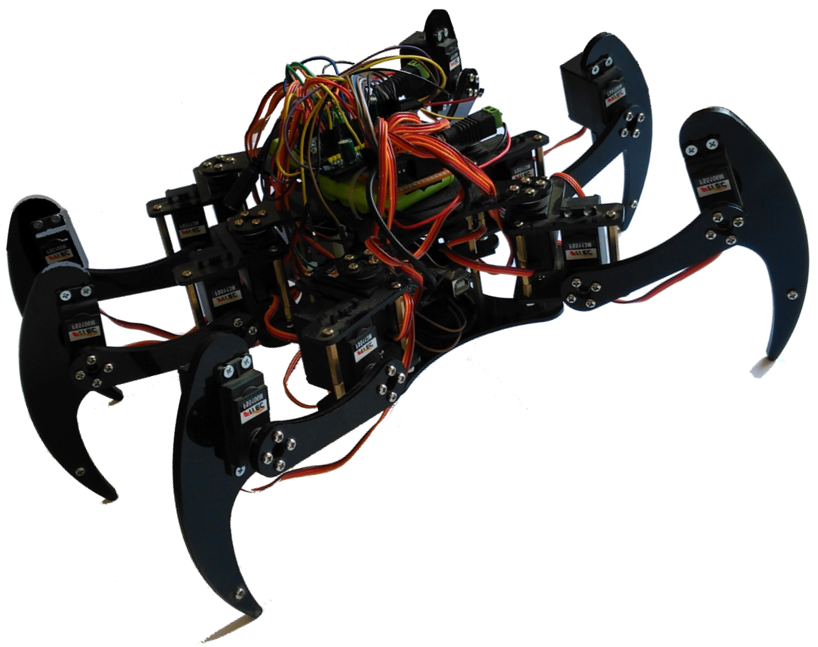
\includegraphics[width =0.8\textwidth]{Fig12}
    \caption{ A sex-legged walking robot.}
    \label{fig1}
\end{figure}

One of the interesting features of hexapod robots such as our ZagHexa (shown in Fig.\ref{fig1}) is that they can climb over obstacles larger than the equivalent sized wheeled or trucked vehicle. In fact, the use of wheels or crawlers limits the size of the obstacle that can be climbed to half the diameter of the wheels. On the contrary, legged robots can overcome obstacles that are comparable with the size of the machine leg\cite{2}. Hexapod walking robots also benefit from a lower impact on the terrain and have greater mobility in natural surroundings. This is especially important in dangerous environments like mine fields, or where it is essential to keep the terrain largely undisturbed for scientific reasons \cite{3}. \\

Hexapod legged robots have been used in exploration of remote locations and hostile environments such as seabed \cite{4}, in space or on planets \cite{5,6}  in nuclear power stations \cite{7}, and in search and rescue operations\cite{8}. Beyond this type of application, hexapod walking vehicles can also be used in a wide variety of tasks such as forests harvesting, in aid to humans in the transport of cargo, as service robots and entertainment. Development of hexapods is increasingly robust in the military sector. Armies all over the world are exploring ways of using hexapods to detect land mines, traverse rocky, unstable terrain, and carry out simple delivery missions in danger zones.

\section{History} 
Robots inspired by insects and other animals have previously been designed with physical antennae and tactile sensors to navigate their environment, as in the work by Brooks (1989) \cite{20,22}, Cowan et al. (2005), Hartmann (2001) \cite{27} and Lee et al. (2008) \cite{10}; the last three works employed the use of a single tactile element rather than a pair \cite{13}.
Because of their extreme mobility and agile adaptability to irregular terrain, insects have long been an inspiration for the designers of mobile and legged robots \cite{11,14}. Early hexapod robots such as Genghis and later creations such as Tarry implemented insect-like mobility based on observations of insect behaviors. The inter- leg coordination system developed by Holk Cruse \cite{30,23}  has been widely implemented   in legged hexapods and its basis is in behavioral experiments that qualitatively analyzed insect walking behaviors \cite{18}.

\subsection{Early Designs}
The first hexapods can be identified as robots based on a rigidly predetermined motion so that
an adaptation to the ground was not possible. Early researches in the 1950s were focused on assigning the motion control completely by a human operator manually\cite{11h}. 
\begin{figure}[h]
    \centering
    \begin{tabular}{ l l }
        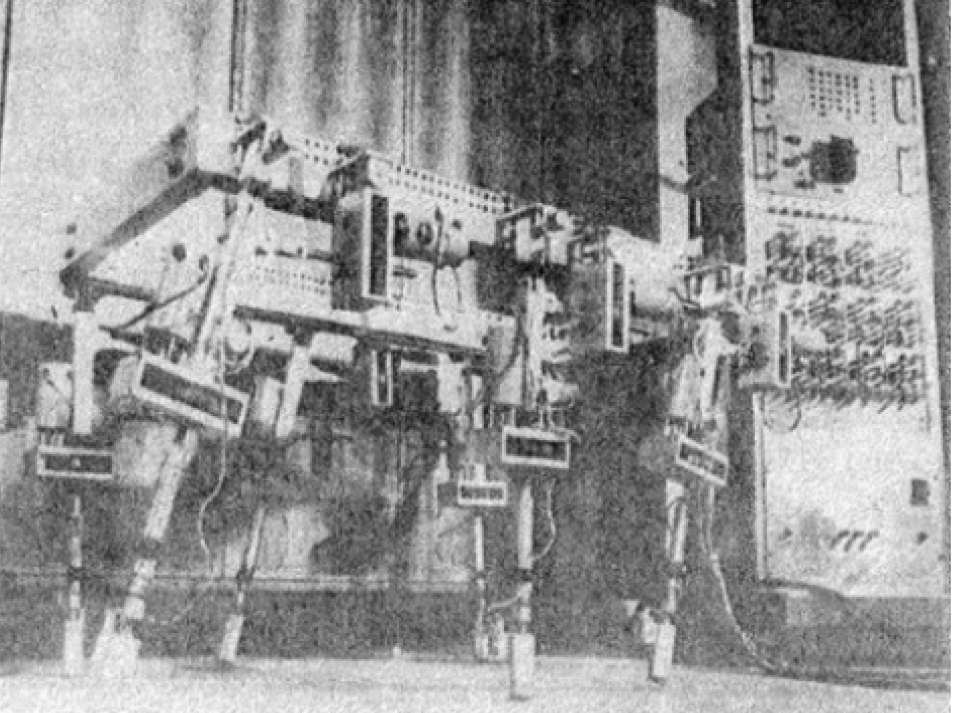
\includegraphics[width =.45\textwidth]{2_a} & 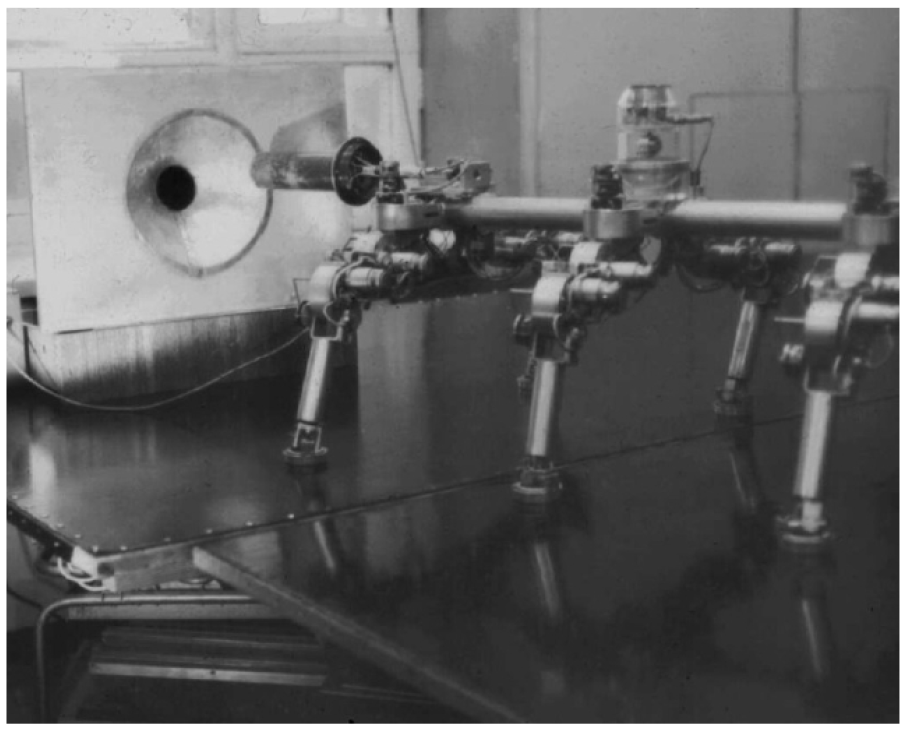
\includegraphics[width =.42\textwidth]{2_b} \\ 
        \hspace{3.5cm}(a) & \hspace{3.3cm}(b)\\
        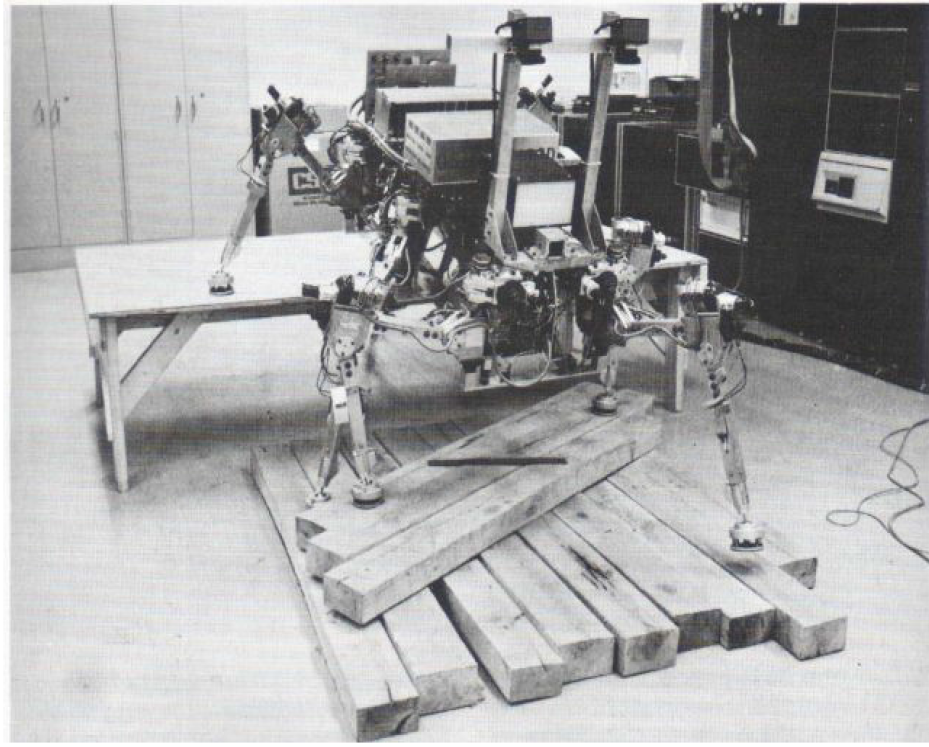
\includegraphics[width =.45\textwidth]{2_c} & \hspace{2cm} 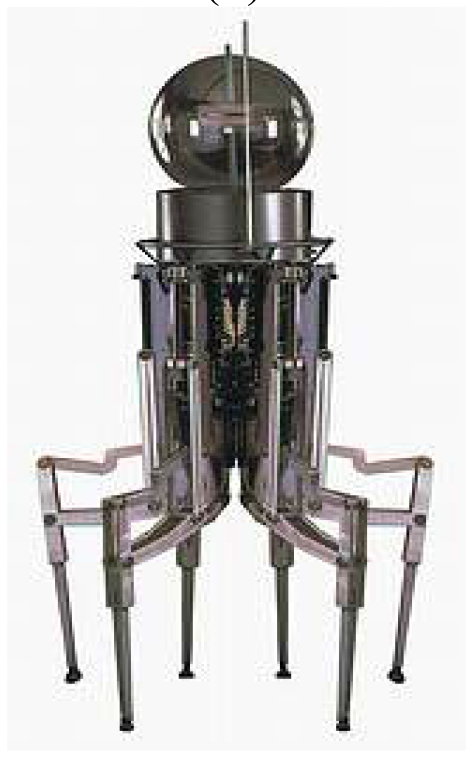
\includegraphics[width =.23\textwidth]{2_d} \\ 
        \hspace{3.5cm}(c) & \hspace{3.3cm}(d)\\
    \end{tabular}
    \caption{Early hexapod design: (a) University of Rome’s hexapod; (b) MASHA hexapod; (c) OSU hexapod; (d) ODEX I hexapod.}
    \label{fig2}
\end{figure}

One of the first successful hexapod robot was constructed at University of Rome in 1972 (Fig.\ref{fig2}a) as a computer-controlled walking machine with electric drives\cite{12h}. In the middle 70s, at the Russian Academy of Sciences in Moscow, a six-legged walking machine was developed with a mathematical model of motion control. It was equipped with a laser scanning range finder and was connected with a two-computer control system \cite{13h}. In 1976, Masha hexapod walking robot was designed at Moscow State University (Fig.\ref{fig2}b). The robot had a tubular axial chassis, articulated legs with three DoFs \cite{14h}. The hexapod was able to negotiate obstacles using contact on the feet and a proximity sensor. Ohio State University in 1977 developed a six-legged insect-like robot system called “OSU Hexapod” \cite{15h}. This hexapod was kept tethered and was made to walk short distances over obstacles (Fig.\ref{fig2}c).
In 1984, Odetic Inc., California, USA, developed Odex I \cite{17h}, a six-legged radially symmetric hexapod robot which used an onboard computer to play back pre-programmed motions (Fig.\ref{fig2}d).


\subsection{Recent Developments}
The two last decades have been characterized by a rapid development of control systems technology. Hexapod robots were equipped with various sensing systems. Artificial Intelligence systems were widely applied to the analysis of environment and motion of robots on a complex surface. A series of bio inspired robots was developed at Case Western Reserve University (USA) at the end the 90s, such as, for example, Robot III that had a total of 24 DoFs. Robot III architecture was based on the structure of cockroach, trying to imitate their behavior \cite{25h}. In particular, each rear leg had three DoFs, each middle leg four DoFs and each front leg five DoFs. Similarly, Biobot was a biomimetic robot physically modeled as the American cockroach (Periplaneta Americana) and powered by pressurized air \cite{26h}. This hexapod had a great speed and agility. \\
Each leg of the robot had three segments, corresponding to the three main segments of insect legs: coxa, femur, and tibia.
\begin{figure}[h]
    \centering
    \begin{tabular}{ l l }
        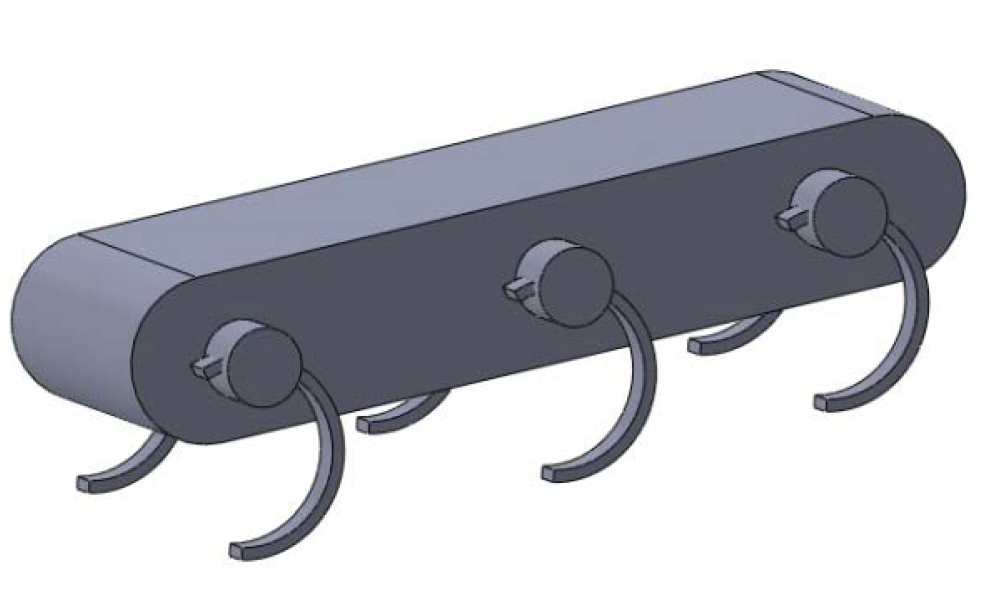
\includegraphics[width =0.45\textwidth,height=0.2\textheight]{3_a} & 
        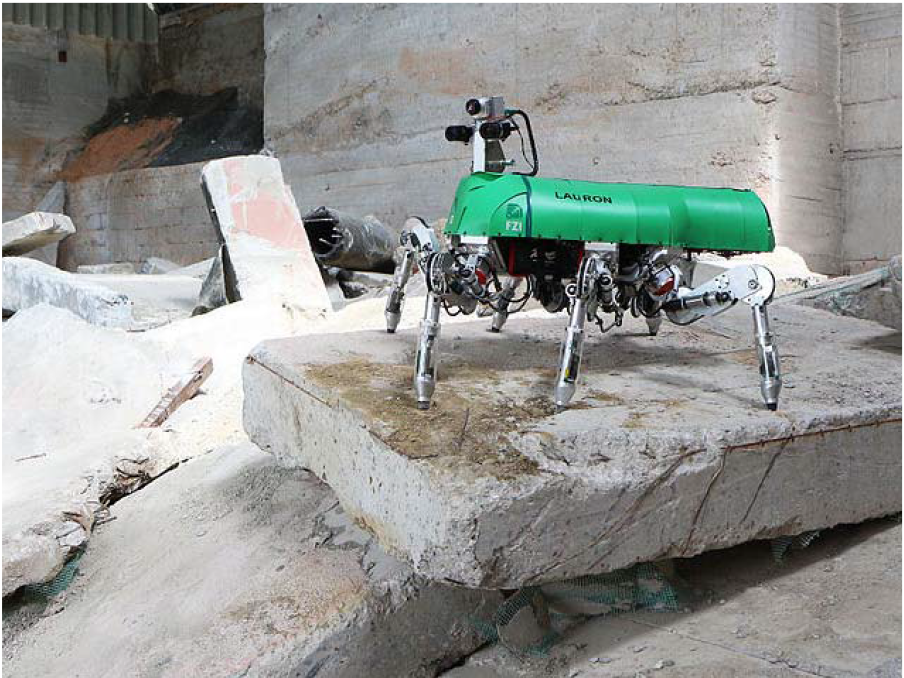
\includegraphics[width =0.45\textwidth,height=0.2\textheight]{3_b} \\ 
        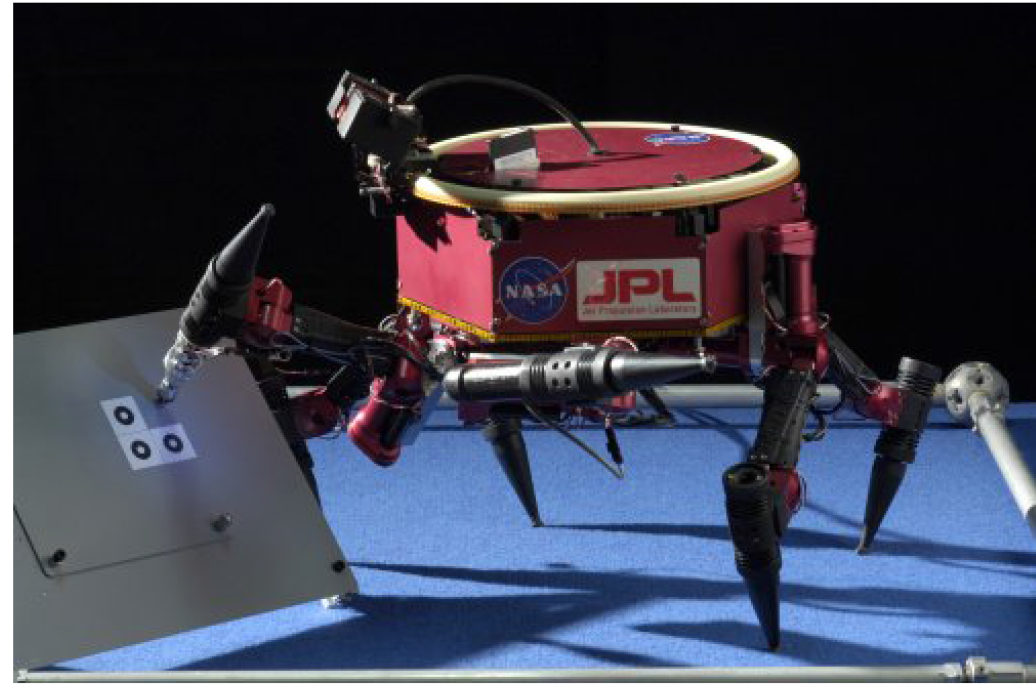
\includegraphics[width =0.45\textwidth,height=0.2\textheight]{3_c} & 
        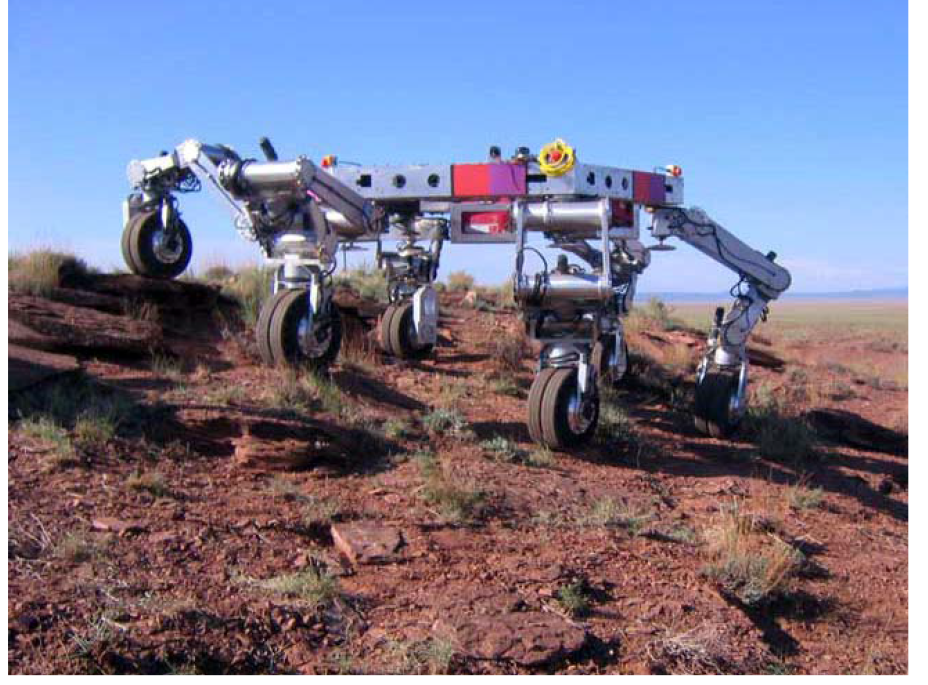
\includegraphics[width =0.45\textwidth,height=0.2\textheight]{3_d} \\ 
    \end{tabular}
    \caption{Some Example on recent developments in hexapod design}
    \label{fig3}
\end{figure}


%%%%%%%%%%%%%%%%%%%%%%%%%%%%%%%%%%%%%%%%%%%%%%%%%%%%%%%%%%%%%%%%%%%%%%%%%%%%%%%

\setchapterpreamble[o]{%
\dictum[Joseph Addison, \textit{(English essayist, poet, and politician, 1672--1719), Spectator, No. 253}]{% source: http://todayinsci.com/A/Addison_Joseph/AddisonJoseph-Quotations.htm
``It is impossible for us, who live in the latter ages of the world, to make observations in criticism, morality, or in any art or science, which have not been touched upon by others. We have little else left us but to represent the common sense of mankind in more strong, more beautiful, or more uncommon lights.''}\vspace{0.1em}}

\chapter{State of the Art}\label{ch:SotA} %and Related Work
%\input{chapters/relatedWork}
%\input{chapters/stateOfArt}
%%%%%%%%%%%%%%%%%%%%%%%%%%%%%%%%%%%%%%%%%%%%%%%%%%%%%%%%%%%%%%%%%%%%%%%%%%%%%%%

\setchapterpreamble[o]{%
    \dictum[Alan Turing, \textit{(British pioneering computer scientist, cryptanalyst,$\cdots$, and philosopher, 1912--1954)}]{%
        ``A computer would deserve to be called intelligent if it could deceive a human into believing that it was human.''}}
\chapter{Architecture Overview} \label{ch:architecture}
%\input{chapters/architecture.tex}
\cleardoublepage
%\input{chapters/ExperimentalPlatform}
%%%%%%%%%%%%%%%%%%%%%%%%%%%%%%%%%%%%%%%%%%%%%%%%%%%%%%%%%%%%%%%%%%%%%%%%%%%%%%%

\setchapterpreamble[o]{%
  \dictum[Abraham Lincoln, \textit{(American 16$^{th}$ President, 1809--1865)}]{%
    ``Be sure you put your feet in the right place, then stand firm.''}}
\chapter{Robot Foot Ground Contact} \label{ch:legSoilContact}
%\input{chapters/ch2StateOfArt/bekker.tex}
%%%%%%%%%%%%%%%%%%%%%%%%%%%%%%%%%%%%%%%%%%%%%%%%%%%%%%%%%%%%%%%%%%%%%%%%%%%%%%%

\setchapterpreamble[o]{%
  \dictum[Stephen Hawking, \textit{(British theoretical physicist, and cosmologist}]{% source: http://todayinsci.com/A/Addison_Joseph/AddisonJoseph-Quotations.htm
    ``Look up at the stars and not down at your feet. Try to make sense of what you see, and wonder about what makes the universe exist. Be curious.''}}
\chapter{Short--Range Embodied Terrain Classification} \label{ch:shortRange}
%\input{chapters/svm}
%%%%%%%%%%%%%%%%%%%%%%%%%%%%%%%%%%%%%%%%%%%%%%%%%%%%%%%%%%%%%%%%%%%%%%%%%%%%%%%

\setchapterpreamble[o]{%
  \dictum[Chuck Norris, \textit{(American martial artist, actor, film producer and screenwriter)}]{%
    ``I think setting a goal, getting a visual image of what it is you want. You've got to see what it is you want to achieve before you can pursue it.''}}
\chapter{Long--Range Visual Terrain Classification} \label{ch:visual}
%\input{chapters/visualClassification}
%%%%%%%%%%%%%%%%%%%%%%%%%%%%%%%%%%%%%%%%%%%%%%%%%%%%%%%%%%%%%%%%%%%%%%%%%%%%%%%

\setchapterpreamble[o]{%
  \dictum[Dr. Seuss, \textit{(American writer and cartoonist, 1904--1991)}]{%
    ``You have brains in your head. You have feet in your shoes. You can steer yourself in any direction you choose. You're on your own, and you know what you know. And you are the guy who'll decide where to go.''}}
\chapter{Path Planning and Following } \label{ch:path}
%\input{chapters/pathPlanningCameraModel}

%%%%%%%%%%%%%%%%%%%%%%%%%%%%%%%%%%%%%%%%%%%%%%%%%%%%%%%%%%%%%%%%%%%%%%%%%%%%%%%

\setchapterpreamble[o]{%
  \dictum[Richard P. Feynman, \textit{(American theoretical physicist, 1918--1988)}]{%
    ``It doesn't matter how beautiful your theory is, it doesn't matter how smart you are. If it doesn't agree with experiment, it's wrong.''}}
\chapter{Experiments and Results} \label{ch:experiments}
%\input{chapters/expEmbodied}
%\cleardoublepage
%\input{chapters/expPathFollow}
%%%%%%%%%%%%%%%%%%%%%%%%%%%%%%%%%%%%%%%%%%%%%%%%%%%%%%%%%%%%%%%%%%%%%%%%%%%%%%%
\setchapterpreamble[o]{\dictum[George Henry Lewes, \textit{( English philosopher and critic of literature, 1817--1878)}]{The true function of philosophy is to educate us in the principles of reasoning and not to put an end to further reasoning by the introduction of fixed conclusions.}}
\chapter{Conclusions and Future Outlook} \label{ch:conclusion}
%This paper presents a system description and the main aspects related to the design, construction, and implementation of six-leg robot named ZagHexa. The robot is a legged robot for search and rescue missions. It benefits form the reliability of its legged locomotion with the flexibility and versatility required to operate in different types of surface. The robot was constructed and tested to walk using tripod, wave and ripple gaits, can rotate and it is equipped with different sensors.

The robot was tested on different surfaces and in rugged terrain. The repeatability of the robot movement as well as the sensor system was also tested.	 These features are mainly achieved due to its original movement that make it deal with different surfaces. Additionally, its shape and weight give it more stability, and its ability to continue with its moving and sensing capabilities after collisions or even small falls. \\ 
However, more tests and experiments to improve and validate the design and sensor performance are to be carried out to optimize the system performance.
Finally, we are working on tackling some issues should to have fully autonomous operation and integration into a heterogeneous system. To make the integration of ZagHexa into different missions easier, an effort is being carried to provide it with a standard connectivity over the ROS framework.
%\input{chapters/futureWork}

%%%%%%%%%%%%%%%%%%%%%%%%%%%%%%%%%%%%%%%%%%%%%%%%%%%%%%%%%%%%%%%%%%%%%%%%%%%%%%%
%\appendix
%%\chapter{Camera Calibration, Model, and Configurations}\label{ch:cameraModel}
%%\input{chapters/appCameraModel}
%\chapter{Software Description}\label{ch:softwareDescription}
%\input{chapters/appsSoftwareDescription}

%%%%%%%%%%%%%%%%%%%%%%%%%%%%%%%%%%%%%%%%%%%%%%%%%%%%%%%%%%%%%%%%%%%%%%%%%%%%%%%
\backmatter %------------------------------------------------------------------
\cleardoublepage{}
\renewcommand{\nomname}{List of Symbols and Abbreviations}
\markboth{\nomname}{\nomname}\printnomenclature{}
\nocite{*}
\bibliographystyle{apalike}
%\bibliography{myPhDreferences,myPublications}
%\cleardoublepage{}
%\printindex{} %\cleardoublepage{}
\end{document}